\chapter{Design and Implementation}
In this chapter we will review in detail the design of our framework and each corresponding module.
We will discuss how modules interact and the reasoning behind the design choices we made.
We will also discuss problems which we encountered when building the framework as well as those that came to light during initial use.
We broke down this chapter into sections stemming from the higher level design concepts into the lower level modules.
This will make it easier to piece together the utility of each module we introduce and its required functionality.
After the sections on the framework itself, we will implement our learning algorithm (MLN).
Finally we will review the process of integrating our learning algorithm with the framework and test its overall functionality.
Results and analysis will be reviewed in the next chapter.
% section{What we are doing}
\section{High level architecture}
Before defining the high level architecture for a platform meant to support the development of learning models, we must review what a common learning architecture looks like.
These are well established, and for our system it represents the core of what needs to be supported in order for the framework implementation to be a viable asset to the community.
This includes architecting for the support of different domains, languages and environments as these core components will later be expanded.
A base learning architecture has three components, input data a learning model and an evaluation tool.
In the case of learning action models, input data can be produced from real or synthetic measures, the learning model will need to output an action model, and the evaluation tool will then use a domain simulator to test the action model for validity and accuracy.
A domain simulator can also in turn be used to produce synthetic data.

\begin{figure}[h]
 \centering

 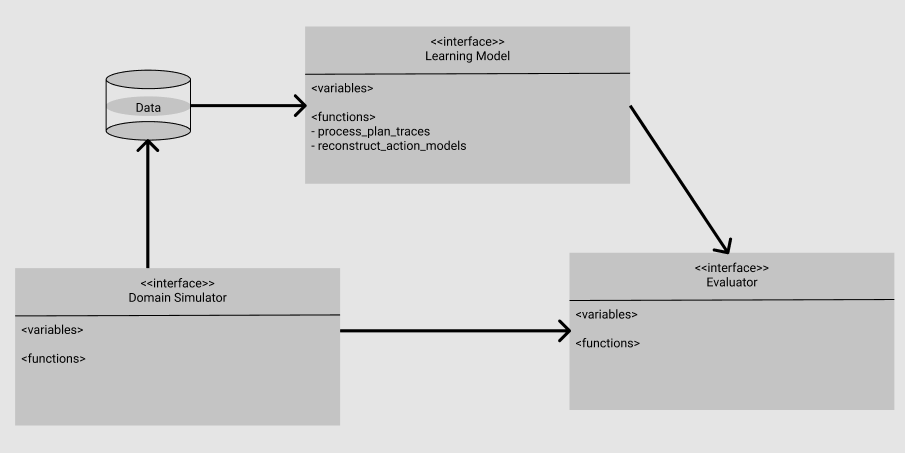
\includegraphics[width=0.7\textwidth]{images/architecture/Core Architecture}
 \caption{Core elements of a learning architecture for reconstructing action models.}

\end{figure}
\newpage
\section{Domain parsing and simulation modules}
\subsection{Parsing module}
For parsing domain languages we implemented the architecture defined in figure \ref{fig:parser-uml}.
Then we proceeded to integrating support for PDDL 2.1 .
The parsing toolkit of choice was Antlr because factors such as ease of use and compatibility with multiple languages made it much easier to develop with.
We could also easily separate a language features/nodes into different files meaning that maintenance and extension of our implementation is much simpler even for people unfamiliar with the structure of modern parsing toolkits.
We followed the BNF Description of PDDL 2.1 defined in \cite{pddl21:online} to ensure compliance with standards.
This also made it easier to test and ensure parsing of each definition was performed correctly.
\begin{figure}[h]
 \centering
 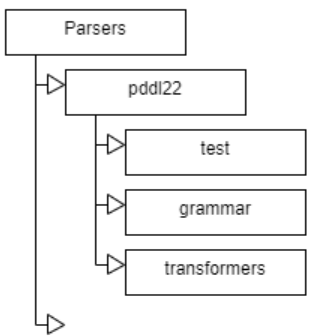
\includegraphics[width=0.3\textwidth]{images/architecture/parser_dir}
 \caption{Directory structure under framework root for integrating parsers.}
  \label{fig:parser-dir}
\end{figure}
\newline
Figure \ref{fig:parser-dir} demonstrates how the integration of new parsers to the framework is done.
We omitted creating an interface layer for transformers with our simulation module as it is unnecessary when working with a single language, and we are interested in an initial proof of concept.
An interface layer was also introduced in order to support for other domain languages in the future, making development much more straight forward.

As of now we based the simulation engine on the semantics defined for the PDDL 2.1 \cite{pddl21:online}.
Rules are extensively defined, and we made sure to separate these in our code allowing for modifications when upgrading for newer versions of PDDL.
Unfortunately this does mean that as of now we have coupled our simulation engine with our parser, however this is only due to the lack of development time invested in this section of the framework.
The disadvantages of this coupling will be evident when attempting to integrate a new parser, as it will have to follow the rules of the engine.
However we do assume that this can be mitigated over time by upgrading and extending the simulation engine to support different input formats and rules therefore making it more generic.
\newpage
To provide an indication of how the parser is implemented we will now provide a vertical slice of a simple lexical component.
Our example will be on the implementation of the predicate in the PDDL 2.1 specification.
The specification states that the predicate is defined as follows:
\begin{lstlisting}
<predicate>     ::= <name>
*** dependencies ***
<name>          ::= /([a-zA-Z]|\d)+((_|-)([a-zA-Z]|\d)+)*/
\end{lstlisting}
With this specification we can define the grammar.lark file for predicate, we assume that all dependencies are satisfied.

\begin{lstlisting}t
%import .name.name

predicate: name
\end{lstlisting}
This demonstrates how simple our chosen architecture is and how flexible the system is to modify. The next step is to specify the transformer that converts predicate nodes into a python data structure for use in the simulator.

\begin{lstlisting}[language=Python]
from lark import Transformer


class Predicate(Transformer):

    @staticmethod
    def predicate(args):
        val = args[0].children[0]
        return val

\end{lstlisting}
Predicate is a relatively simple structure so we only need to recover the stored underlying value of "name" as they are both strings, more complicated structures such as actions, depend on more complex implementations that align with their use cases.
Finally we test the parser to ensure that it performs as expected given the data we would reasonably expect to pass it:


\newpage
\begin{lstlisting}[language=Python]
import os
from unittest import TestCase
from lark import Lark
from pddl_parser.transformers import Predicate

class TestGrammarPredicate(TestCase):
    def setUp(self) -> None:
        self.grammar = """
        start:predicate
        %import .predicate.predicate
        %import common (WS)
        %ignore WS
        """
        self.transformer = Predicate()
        self.import_path = [f'{os.getcwd()}/../../grammar/']
        self.parser = "lalr"

    def test_predicate_parses_kebab_case(self):
        try:
            parser = Lark(grammar=self.grammar, import_paths=self.import_path, parser=self.parser)
            parser.parse("""predicate-with-dashes""")
        except Exception as e:
            self.fail(msg=e)

    def test_predicate_parses_snake_case(self):
        try:
            parser = Lark(grammar=self.grammar, import_paths=self.import_path, parser=self.parser)
            parser.parse("""predicate_with_underscores""")
        except Exception as e:
            self.fail(msg=e)

    def test_predicate_parsing_fails(self):
        parser = Lark(grammar=self.grammar, import_paths=self.import_path, parser=self.parser)
        self.assertRaises(Exception, parser.parse, """space separated""", msg='failed to raise on space separator')
        self.assertRaises(Exception, parser.parse, """(not-char""", msg='failed to raise on non char in word')
        self.assertRaises(Exception, parser.parse, """1not-num""", msg='failed to raise on num in word')

    def test_predicate_transformer(self):
        try:
            parser = Lark(grammar=self.grammar, import_paths=self.import_path, transformer=self.transformer,
                          parser=self.parser)
            parser.parse("""predicate-with-dashes""")
        except Exception as e:
            self.fail(msg=e)
\end{lstlisting}
We can observe that tests are more extensive as we want to ensure that when using our parser unwanted behaviour does not occur.
Code is only ever as good as the tests supporting it because when modifications are made, only tests can assure a developer that other features have not been compromised and if they have, then there are clear steps to fixing them.

\subsection{Simulation module}
The simulation module relies on being populated by an initial state conforming to a json standard as of now defined by the Parsing module.
A domain is parsed and converted to a json representation which is easier to manage.
Actions are then initialised from the parsed domain and an initial state is populated from a parsed problem file.
The simulator at this time permits the execution of actions and the tracking of changes in the state.
This functionality although relatively rudimentary has been sufficient for the purpose of producing plan traces and verifying if simple actions performed correctly when generated by the learning model.

\begin{lstlisting}[language=Python]
class State:
    def __init__(self, state:dict):
        self._actions = dict()
        self.actions = state["actions"]
        self.state = set()
        self.latest_removed = set()
        self.latest_added = set()
        # self.latest_added=set()

    @property
    def actions(self) -> dict:
        """
        Actions that can be performed on the domain state.
        """
        return self._actions

    @actions.setter
    def actions(self, actions: list):
        """
        Setter for actions of the state, must a list of json dictionaries.
        """
        for a in actions:
            self._actions[a["name"]] = Action(**a)

    def perform_action(self, p: Predicate):
        """
        Perform an action in the format of Predicate ( "name(*v)") on the state.
        :raises KeyError if action does not exist.
        """
        pos = self.actions[p.name].get_pos_list(p.args)
        self.state = self.state | pos
        self.latest_added = pos
        neg = self.actions[p.name].get_neg_list(p.args)
        self.latest_removed = neg
        self.state = self.state - neg

    def set_init_state(self, predicate_json):
        """
        Populates initial states with predicates
        """
        for p in predicate_json:
            self.state.add(Predicate(**p))
\end{lstlisting}

The above is a simplified version of the Simulation module, it provides a bare-bones PDDL action simulator.
As problems become more complex and simulation needs to support more functionality, this module can be expanded and eventually integrated with third-party tools such as Unity (for simulating 3d models) or Gazebo with ROS (robot operating system) to view how a state changes in real time.
Performing an action and testing if a goal state has been reached is very intuitive which is helpful for legibility and use.


\newpage

\section{Learning model interface and implementation}
The learning model interface defines the class interaction that is required for the full implementation of a learning model.
We are only displaying the UML nearest neighbours as previously mentioned in order to best demonstrate the functionality required by the module we are working with.
\begin{figure}[h]
 \centering
 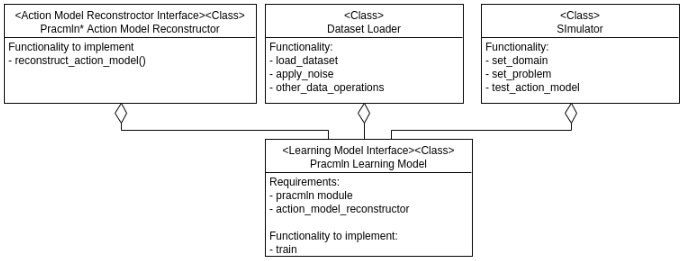
\includegraphics[width=1\textwidth]{images/architecture/learning_module_interaction_uml}
 \caption{Learning model class dependency UML.}
  \label{fig:learning-module-interaction-uml}
\end{figure}
\newline
The above figure displays how we have implemented a sample learning model.
For the implementation of the train function we have full use of the dataset loader to get the necessary data and perform any transformation on it.
The dataset loader is similar to a library like Pandas, providing the ability to load data in the correct format from files.
This was a necessary implementation in our use case are defined differently from standard numpy arrays.
We previously defined the data generation interface, this interface ensures that data is compatible with our dataset loader and is flexible enough for any use by the implemented learning model.
The learning model can also make use of the simulator to test if the predicted action model is valid and how well it performs on given problems.
This can be used as part of the optimization function when training, although we have tested this to date.

The code associated with this module is provided to the user under name of "learn".
The base interface as of this moment is as follows:
\begin{lstlisting}[language=Python]
from abc import abstractmethod

class LearningModelInterface:
    def __init_subclass__(cls, **kwargs):
        pass

    @abstractmethod
    def train(self):
        ...
\end{lstlisting}
We can observe that the interface any new learning model classes must conform to is relatively lax.
This approach was taken in order to provide as much freedom to the developer as possible until more robust standards are put in place.
The implementation for the pracmln learning model which we have implemented follows the above specification and is available for public use.
This class signature also provides a familiar interface for users using models in all common ML libraries, the train function is very well known and abstracts the complex inner workings of a learning algorithm away.

Here is our sample implementation for the pracmln learning module using a StateInference object to manage databases and the MarkovNetworks being generated:
\begin{lstlisting}[language=Python]
import os
import random

from collections import defaultdict
from learn import LearningModelInterface
from .state_inference import Database as DB
from .state_inference import StateInfrence
from .utils import load_dbs


class PracmlnLearningModel(LearningModelInterface):
    def __init__(
            self,
            mln_database_path: str,
            domain_p_decs_path: str,
            max_databases=25,
    ):
        # load dataset
        databases = load_dbs(mln_database_path)
        random.shuffle(databases)
        databases = databases[:max_databases]
        self.dataset = [DB.parse_db(db) for db in databases]

        # initiate pracmln learner
        self.state_inference: StateInfrence = StateInfrence(
            os.path.normpath(os.path.join(os.getcwd(), domain_p_decs_path))
        )

    def train(self):
        # track how many databases were added for each action being learnt
        opt_tracker = defaultdict(int)
        for i, d in enumerate(self.dataset):
            # pass data through Markov Logic Network
            self.state_inference.process_database(d)
            opt_tracker[d.action.name] += 1
            # write data for metrics, remove for speed & space use reduction
            self.state_inference.save_data_for_graphing()
        # plot learning confidence results.
        self.state_inference.plot()
\end{lstlisting}
This sample of code provides an example of the freedom provided when developing a custom learning module.
Having the flexibility provided facilitates experimental use and design whilst conforming to a bare minimum of standards which are necessary for legibility and wider adoption.
The simplicity of using this interface will be highlighted when the sample project demonstrated.
The detail for the inner workings such as dataset structure and training of the MLN learning module are specified in the next chapter.

\newpage
\section{Integrating MLN Learner module}
A STRIPS domain consists of a state \(S\) and a set of action models \(M\).
\(S\) is a set of predicates with typed arguments.
A strips action model \(A\) which we are attempting to reconstruct, is defined by  \(\{a,a_{pre},a_{add},a_{del}\}\). \(a\) is the name with typed arguments of the function, \(a_{pre}\) is set of preconditions which specify the conditions of a state under which \(a\) can be applied. \(a_{add}, a_{del}\) is the add and delete list respectively, these lists indicate the effects of \(a\) on a state, specifying which new predicates are to be added and which existing predicates are to be removed.
\newline \newline
We define a valid database \(D\) by \(\{a,S_{p}\}\) where \(S_p\)  is a set of predicates in the form \(p_{name}(p_{args},f\in \{-1,0,1\})\), the modification here is that we have added a variable \(f\) to each predicate representing if it is a member of \(a_{add}\) if \(f=1\), \(a_{del}\) if \(f=-1\) and the set of predicates where \(f=0\) form a super-set of \(a_{pre}\).
\newline \newline
A plan with its intermediate state-action pairs can hence be represented as an ordered list of databases. This representation is useful because it allows us to now create a model which predicts \(A\) given a partially complete database after training.
\newline \newline
In order to tackle possible noise in the database we need to use a model that can handle constraints being violated, one such model is a Markov Logic Netork (MLN). Where as a first-order knowledge base is a set of hard constraints on a set of possible worlds in which a violation of a constraint implies 0 probability for said world. MLN's soften these constraints and reduces the weight of the violating constraint making the world less probable instead of impossible. MLN's are formulated as a set of pairs \(w_i,F_i\) where \(w_i\) is the weight of a formula represented as a real number, and \(F_i\) is a formula in first-order logic. Together with a finite set of constraints \(C = \{c_1,c_2,...,c_{|C|}\}]\), it defines Markov network \(M_{L,C}\) as follows:
%ref: https://homes.cs.washington.edu/~pedrod/kbmn.pdf
% equation 1
% equation 2
\section{Training and reconstruction of STRIPS action models}
Strips action models can be reformulated as a conjunction of typed predicates \(a_{pre},a_{add},a_{del}\), this set of predicates belonging to a specific action should represent a subset of a database for a matching action. As we have no prior knowledge of the valid subset when creating and training the MLN, we must assume that all predicates a valid and generate an MLN accordingly. Once weights reduce bellow a set threshold we can prune them out of the MLN as they represent predicates that would render the action model improbable.
    \newline \newline

The algorithm for generating and training an MLN from a database instance is as follows:

\newline
process \(D\):\newline
\(MLN \impliedby action\_MLNS[a] \) \newline
for each predicate \(p\) that has not been pruned or previously added to \(MLN\):\newline
----- generate and add formula: \(a \implies p\) with initial weight 0 to \(MLN\)\newline
train MLN (online)  with database \(D\)\newline
prune weights (for efficiency)\newline

once training is complete we can extract each predicate with its weight .

An optimization for the above routine is to prune any predicates that does not share variables with the action being processed.

Due to a lack of resources available for working with PDDL in python, I have designed a system for generating generic plan traces from PDDL in python. This was necessary as many modern learning tools use python and it is a language that saves a lot of development time thanks to readily available complex libraries (Tensorflow, Pracmln, Pytorch, Sklearn etc...). Such libraries will allow for more interesting strategies in tackling the problem at hand. \newline \newline
The greatest difficulty encountered is in the Generation of Plan Traces, as planners used don't provide intermediate states or add and delete lists, hence these must be generated from the parsed action models directly. There are no known libraries for parsing action models that support more than simple STRIPS, hence a custom extendable parser was
implemented.


\newpage
\section{Evaluation module}
The purpose of this module is to leverage the simulator and the output action model from training to evaluate its performance given the desired functionality set by the user.
The functionality includes a given domain and a set of problems which cover the scenarios the action model will be subjected to.
The functionality desired by the user may also include specific responses to pre-defined states if such states are encountered in the domain as the plan is being executed.

\newpage
\section{Final integration}
\begin{figure}[h]
 \centering
 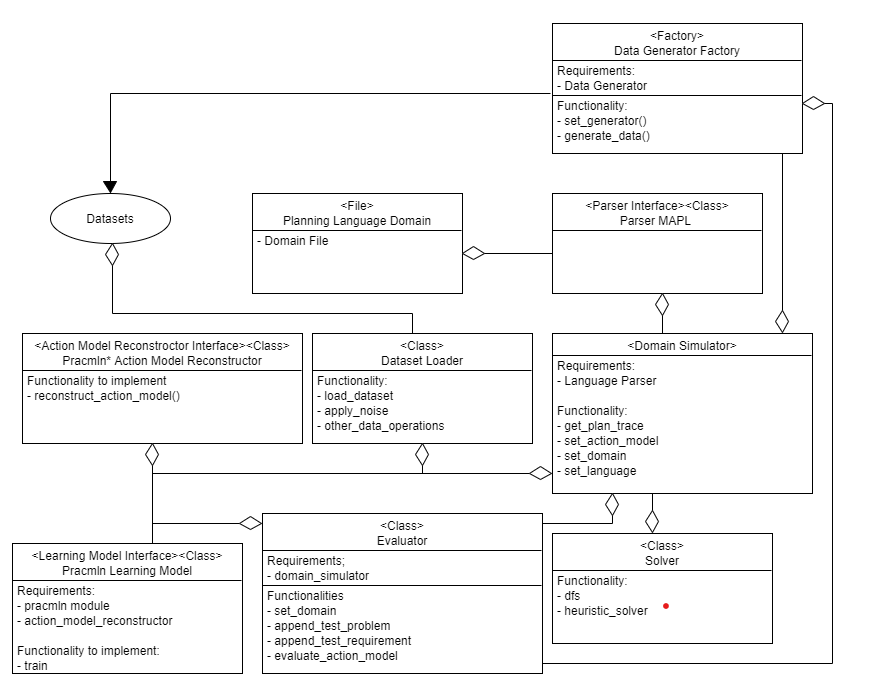
\includegraphics[width=1\textwidth]{images/architecture/final_integration_uml}
 \caption{Relations of most important modules for complete framework for a specific use-case, ignoring interfaces}
  \label{fig:learning-module-interaction-uml}
\end{figure}
In the figure above, we display the interaction between all important modules for our use case. This ignores the interfaces we provided for other languages, domains, data generators and learning models that can be added seamlessly to the framework. We can observe the end to end flow of data, from the initial generation of training datasets, to the training of prediction models and their evaluation.


As all of the necessary modules have now been defined, we can demonstrate a sample project that specifies a specific domain, generates a dataset, trains a model on this dataset and finally evaluates the trained model:

\begin{lstlisting}[language=Python]
import os

from generator.generator import GridWorldGenerator
from solvers.solvers import FFXSolver
from learn.pracmln_learning_model.utils import write_dbs
from learn.pracmln_learning_model import PracmlnLearningModel
from learn.pracmln_learning_model.utils import MLNDeclarationGenerator

BASE_PATH = os.path.normpath(f"{os.getcwd()}/..")

PROJECT_DIR = os.path.dirname(__file__)
DATA_DIR = f"{PROJECT_DIR}/data"
PROBLEM_STATE_DSET_DIR = f"{DATA_DIR}/problem_states"
DOMAIN_FILE = f"{PROJECT_DIR}/grid.pddl"
PROBLEM_SOLUTION_DIR = f"{DATA_DIR}/problem_solutions"
MLN_DATABASE = f"{DATA_DIR}/mln_db.mln"
DOMAIN_P_DECS = f'{DATA_DIR}/mln_grid_p_decs.txt'
# generate problem dataset
GridWorldGenerator.generate_data(output_dir=PROBLEM_STATE_DSET_DIR)
# generate solutions dataset
FFXSolver.solve_problem_dir(
    domain_file=DOMAIN_FILE,
    problem_dir=PROBLEM_STATE_DSET_DIR,
    output_dir=PROBLEM_SOLUTION_DIR,
)
# simulate solutions to generate plan trace dataset (mln_db)
write_dbs(
    domain_file=DOMAIN_FILE,
    problem_state_dir=PROBLEM_STATE_DSET_DIR,
    problem_solution_dir=PROBLEM_SOLUTION_DIR,
    mln_db_path=MLN_DATABASE,
)
# generate necessary mln predicate declarations
MLNDeclarationGenerator.gen(DOMAIN_FILE, DOMAIN_P_DECS)
# instantiate and train model
model = PracmlnLearningModel(mln_database_path=MLN_DATABASE, domain_p_decs_path=DOMAIN_P_DECS)
model.train()
\end{lstlisting}

From the above code we can observe how comfortable the process is from generating necessary data, simulating a pddl domain state to training a model.
The simplicity and modularity being a key aspect of our design goals can be clearly observed.
An initial dataset of 100 problems is generated for the specified domain.
A specified solver in this cas FFX generates a solutions dataset given our problems and domain.
The Simulation module generates plan traces from the solutions and problems and creates a dataset of MLN databases for the learning model.
Finally the learning model processes these databases and traines a markov network for each action present in the dataset.

%  Existing  techniques for learning action traces...

%  define error for preconditions

% extrapolate to error of action model.




% Encoding of action plan trace (Database)

% Encoding of a logic network
% Training of a logic network
% Noise
% Prediction
% Error evaluation
